\documentclass[conference]{IEEEtran}

\usepackage{graphicx}
\usepackage{amsmath}
\usepackage[caption=false,font=footnotesize]{subfig}
\usepackage{url}
\usepackage[numbers]{natbib}

\begin{document}


\title{PANDORA Monstertruck: A 4WS4WD Car-Like\\Robot for Autonomous Exploration in\\Unknown Environments}


% author names and affiliations
\author{\IEEEauthorblockN{George Kouros}
\IEEEauthorblockA{Department of Electrical and Computer Engineering\\
Aristotle University of Thessaloniki\\
Thessaloniki, Greece\\
Email: gkourosg@yahoo.gr}
\and
\IEEEauthorblockN{Loukas Petrou}
\IEEEauthorblockA{Department of Electrical and Computer Engineering\\
Aristotle University of Thessaloniki\\ Thessaloniki, Greece\\
Email: loukas@eng.auth.gr}}

%\IEEEspecialpapernotice{(Invited Paper)}
% make the title area
\maketitle

\begin{abstract}
This paper presents a four-wheel-steering four-wheel-drive (4WS4WD) car-like robot, able to autonomously explore unknown environments with flat or uneven terrain. The robot uses a set of sensors and actuators and employs a number of algorithms to effectively map the environment, localize in it, plan and execute motions while utilizing the maneuverability of the four-wheel-steering kinematic model. For the task of autonomous navigation, a ROS-based 4-Tier architecture is proposed consisting of global path planning, dynamic local path deformation for collision avoidance, kinematically feasible local path synthesis and finally path tracking control using a fuzzy logic controller for 4WS car-like robots.
\end{abstract}


\section{Introduction} \label{sec:introduction}
Autonomous Mobile Robots (AMR) are robots able to perform tasks without any human intervention or control. AMRs are increasingly used in commercial, industrial, military and lately even domestic settings and are extensively researched worldwide. The AMR presented in this paper, was specifically developed for research purposes in the field of Unmanned Search and Rescue (USAR).

An AMR must be able to perceive its environment, move safely and efficiently inside it and make decisions based on sensory input and artificial intelligence algorithms about how to proceed in order to complete a given task. Therefore, it utilizes a set of algorithms that can be separated into three basic categories, which are perception, decision making and motion planning \& execution. In this particular case, those categories translate to simultaneous localization and mapping (SLAM), exploration (target selection) and autonomous navigation respectively.

This paper presents the architecture of an AMR and the algorithms required for its autonomous operation, focusing on motion planning and execution, while the problems of simultaneous localization and mapping (SLAM) and exploration are tackled, by utilizing a number of open source algorithm implementations. In particular, CRSM-SLAM \cite{crsm} is used to construct a 2D map of the environment and localize in it, while exploration is achieved using a frontier exploration algorithm, which selects a frontier to explore based on an objective function that  takes into account the distance and orientation difference to each frontier, as well as its size and reachability.

The developed robotic platform adheres to a four-wheel-steering kinematic model, which presents a set of nonholonomic constraints that restrict the feasible velocities of the robot in the plane and as a result render the problem of motion planning especially difficult in comparison with the more popular Differential, Skid-Steer and Omnidirectional kinematic models. As a result, the open source implementations of navigation algorithms using Dijkstra and A* graph search for path planning and the Dynamic Window Approach \cite{dwa} or Elastic Band \cite{eband} for collision avoidance and path tracking, should be modified. The employed navigation system architecture follows the same structure as the aforementioned one, but features a collision avoidance and path tracking component that considers the kinematic constraints of the 4WS robot.

The proposed Reeds-Shepp Band method was based on the Nonholonomic Bubble Band by Khatib et al. \cite{dpm}, which dynamically deforms a global path, while satisfying the nonholonomic constraints of car-like robots. The proposed method uses a two-step approach to dynamically deform the global path for collision avoidance using the Elastic Band algorithm and then perform interpolation on the deformed path waypoints using collsion-free Reeds-Shepp paths \cite{reeds_shepp} in order to achieve the kinematic feasibility of the path. The navigation system is complemented with a fuzzy path tracking controller, based on the methods presented in \cite{flc_thesis} for car-like robots and \cite{reactive_fuzzy_ptc} for 4WS robots and aims to take advantage of both the counter steering and crab steering capabilities of the robot.

In Section \ref{sec:robot}, the developed PANDORA Monstertruck robotic platform is presented.  Section \ref{sec:autonav} focuses on the software architecture of the robot and the proposed autonomous navigation system. Section \ref{sec:results} demonstrates the experimental results from simulation and physical robot operation, followed by the conclusions and future work in Section \ref{sec:conclusions}.

\section{The PANDORA Monstertruck Robot} \label{sec:robot}
The PANDORA Monstertruck robotic platform that is depicted in Fig. \ref{fig:monstertruck} was built using a Redcat Racing Groundpounder 1:10 RC monstertruck, that features simultaneous and independent front and rear wheel steering (4WS), as well as drive transfer to all four wheels (4WD).

\begin{figure}[!ht]
	\centering
	\includegraphics[width=0.46\linewidth]{Figures/monstertruck3.png}
	\caption{PANDORA Monstertruck.}
	\label{fig:monstertruck}
\end{figure}

\subsection{Actuators and Motion Transfer}
\subsubsection{Drive System}
The driving motion of the wheels is generated by a single brushless $18000\, rpm$ maxon EC-max 283858 motor, controlled by a maxon EPOS 24/1 positioning controller. The turning motion of the motor is transferred to the wheels via a drivetrain mechanism, as shown in Fig. \ref{fig:drivetrain}, which consists of four basic transfer stages: the motor gearbox (1:66), the spur \& pinion gears (1:1.76), the 4WD transfer case (1:1.68) and the front and rear differentials (1:3.3), resulting in a 1:644 transfer ratio and a maximum speed of $0.2m/s$.

\subsubsection{Steering System}
The steering motion of the wheels is generated by two Hitek HS-7954TH servo motors, controlled by a Pololu Micro Maestro 6-Channel USB servo controller. The servos steer the front and rear wheels via two drag link steering mechanisms, as depicted in Fig. \ref{fig:drag_link_steering}.

\begin{figure}[!ht]
	\centering
	\subfloat[The 4WD drivetrain that transfers the motion from the motor the four wheels.]{
		
\includegraphics[width=0.8\linewidth]{Figures/drivetrain.png}
		\label{fig:drivetrain}}\\[-0.05cm]
	\subfloat[The drag-link-steering mechanism used for the 4WS system.]{
		\includegraphics[width=0.8\linewidth]{Figures/my_drag_link_steering.png}
		\label{fig:drag_link_steering}}%
	\caption{The motion transfer systems of PANDORA Monstertruck.}
\end{figure}

\subsection{Hardware Components}
The main goal of the developed robotic platform is to autonomously explore unknown environments with flat or uneven terrain. In particular, the robot must be able to map its environment and detect obstacles. These tasks are accomplished using a Hokuyo URG-04LX Laser Scanner (Fig. \ref{fig:laser}) that offers laser scans, with a 10Hz frequency, $60-4095mm$ range and $240^\circ$ measurement area.

Reliable localization, mapping and obstacle detection demands the laser scanner to always be stabilized on the horizontal level. This is accomplished by employing a roll-pitch stabilization mechanism consisting of two Dynamixel AX-12A smart servos in a roll-pitch topology (Fig. \ref{fig:stabilizer}) that continuously correct the roll and pitch deviations of the sensor.

The laser scanner stabilization task requires the knowledge of the pitch and roll deviation angles in order to adjust the mechanism rotations using the inverse angles. The roll and pitch angles are measured using a compass and specifically an Ocean Server Compass OS4000 (Fig. \ref{fig:compass}), which contains a 3-axis magnetometer and a 3-axis accelerometer and offers measurements of the $roll$, $pitch$ and $yaw$ angles, as well as the linear accelerations $\alpha_x, \alpha_y, \alpha_z$.

In addition, the sensor equipment of the robot is complemented with a Logitech Portable Webcam C905 (Fig. \ref{fig:webcam}), used at the time, only for monitoring purposes during the teleoperated and autonomous operation of the robot.

Finally, the central node that acts as the brain of the robot and communicates with the sensors and actuators, consists of an ODROID-XU4 single board computer (Fig. \ref{fig:odroid}) that was chosen due to its small size, low power consumption and adequate processing power.

\begin{figure}[!ht]
	\centering
	\subfloat[Laser Scanner]{\includegraphics[height=2cm]{Figures/hokuyo.jpg}\label{fig:laser}}%
	\hspace{0.7cm}	
	\subfloat[Stabilizer]{\includegraphics[height=2cm]{Figures/stabilizer.png}\label{fig:stabilizer}}%
	\hspace{0.7cm}	
	\subfloat[Compass]{\includegraphics[height=2cm]{Figures/compass.jpg}\label{fig:compass}}\\
	\subfloat[Webcam]{\includegraphics[height=2cm]{Figures/webcam.jpg}\label{fig:webcam}}%
	\hspace{0.8cm}
	\subfloat[ODROID-XU4]{\includegraphics[height=2cm]{Figures/odroid-xu4.jpg}\label{fig:odroid}}%
	\caption{The sensors, laser scanner stabilizer and computer board of PANDORA Monstertruck.}
\end{figure}

% lidar, imu, camera
\subsection{Kinematics}
In \cite{vehicle_dynamics} the 4WS kinematic model is presented with the constraint that in order for a 4WS vehicle to perform slip-free motion in low speeds, it must comply with the 4WS Kinematic Condition. This condition states that the perpendicular lines to each wheel must intersect at the same point $O$, called the Instantaneous Center of Rotation (ICR) and is expressed as

\begin{equation}
	\frac{1}{\cot{\delta_{of}} - \cot{\delta_{if}}} + \frac{1}{\cot{\delta_{or}} - \cot{\delta_{ir}}} = \frac{l}{w}
	\label{eq:4ws_condition}
\end{equation}

\noindent
where $\delta$: steering angle, $i$: inner, $o$: outer, $f$: front and $r$: rear, $l$: wheelbase and $w$: track.

However, the developed robotic platform uses steering mechanisms that do not comply with the above kinematic condition and define a steering relation between the left and right wheels that is approximated as equal ($\delta_{if}=\delta_{of}=\delta_f$, $\delta_{ir}=\delta_{or}=\delta_r$). As a result, the wheels are subjected to slipping by their corresponding side-slip angle $\alpha$ ($\alpha_{if}, \alpha_{of}, \alpha_{ir}, \alpha_{or}$), even in low speeds. The slipping of the wheels is demonstrated in Fig. \ref{fig:4ws_slip_model} and is expressed as

\begin{equation}
	\begin{split}
	&\frac{1}{\cot(\delta_{of} - \alpha_{of}) - \cot(\delta_{if} + \alpha_{if})} -\\ &\;\;\;\;\;\;\;\;\;\;\;\;\;\;\;\;\;\;\;\;\;\;\;\;\frac{1}{\cot(\delta_{or} - \alpha_{or}) - \cot(\delta_{ir} + \alpha_{ir})} = \frac{l}{w}
	\end{split}
	\label{eq:monst_kinematic_condition}
\end{equation}
	
\begin{figure}[!ht]
	\centering
	\includegraphics[width=\linewidth]{Figures/monst_slip_model.png}%
	\caption{The 4WS Kinematic Model with Slipping.}
	\label{fig:4ws_slip_model}
\end{figure}

\begin{figure}[!ht]
	\centering
	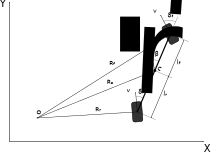
\includegraphics[width=0.7\linewidth]{Figures/4ws_xy_plane.png}%
	\caption{Equivalent bicycle model of the 4WS model on the plane.}
	\label{fig:4ws_xy_plane}
\end{figure}

The motion of the robot in the plane, that is the linear and angular velocities $\dot X, \dot Y, \dot\Theta$, as shown in Fig. \ref{fig:4ws_xy_plane}, using the equivalent bicycle model, can be expressed using the velocity equations from \cite{4ws_trajectory_planning}:

\begin{gather}
	\dot X = v_c \cdot \cos(\theta + \beta)
	\label{eq:x_dot}\\
	\dot Y = v_c \cdot \sin(\theta + \beta)
	\label{eq:y_dot}\\
	\dot \Theta = \omega_c = \frac{v_c \cdot \cos{\beta} \cdot (\tan{\delta_f - \tan{\delta_r}})}{l}
	\label{eq:th_dot}
\end{gather}

\noindent
where $\upsilon_c$ is the resultant speed of the robot and $\beta$ is the sideslip angle and are expressed by
\begin{gather}
	v_c = \frac{v_f \cdot \cos{\delta_f} + v_r \cos{\delta_r}}{2 \cdot \cos{\beta}}
	\label{eq:v_c_f_r}\\[0.1cm]
	\beta = \arctan{\frac{l_r \cdot \tan{\delta_f} + l_f \cdot \tan{\delta_r}}{l}}
	\label{eq:beta}
\end{gather}

\bigskip
\section{Autonomous Navigation in Unknown Environments} \label{sec:autonav}
\subsection{Software Architecture}
The software of PANDORA Monstertruck was based on the Robot Operating System (ROS) and as shown in Fig. \ref{fig:component_diagram} consists of six basic components, as described below.

\begin{figure}[!ht]
	\centering
	\includegraphics[width=\linewidth]{Figures/component_diagram.png}%
	\caption{A simplified component diagram of the software architecture of PANDORA Monstertruck.}
	\label{fig:component_diagram}
\end{figure}


\subsubsection{Hardware-Software Interface}
Component that contains drivers and ROS interfaces for sensors and actuator controllers.
\subsubsection{Control}
Component responsible for teleoperation, the laser scanner stabilization and velocity command priority multiplexing, between navigation and teleoperation commands.
\subsubsection{SLAM}
Component responsible for environment mapping and state estimation using the CRSM-SLAM algorithm.
\subsubsection{Robot State}
Component responsible for publishing the transformations between the reference frames of the joints of the robot.
\subsubsection{Visualization}
Component responsible for the visualization of the information provided by the sensors and algorithms of the robot (runs on the remote monitoring station).
\subsubsection{Navigation}
Component responsible for the exploration and autonomous navigation of the robot. It consists of two nodes, a frontier exploration node for autonomous target selection and the ROS node move\_base, which, given a goal in the world, will try to reach it. The node move\_base, as shown in Fig. \ref{fig:move_base}, is used in combination with the global\_planner plugin and the rsband\_local\_planner plugin, which implement the algorithms Dijkstra/A* for global path planning and the Reeds-Shepp Band algorithm for dynamic local path planning, respectively. The rsband\_local\_planner plugin, also, implements a fuzzy path tracking controller for 4WS car like robots that along with the Reeds-Shepp Band algorithm are presented in the following subsections.

\begin{figure}[!ht]
	\centering
	\includegraphics[width=\linewidth]{Figures/move_base_3.png}%
	\caption{The ROS move\_base node with the global\_planner and\;\;\;\;\;\;\;\;\;\;\;\;\;\;\;\;\;\; rsband\_local\_planner plugins.}
	\label{fig:move_base}
\end{figure}

\subsection{Reeds-Shepp Band}
The proposed Reeds-Shepp Band algorithm is an approximation of the Nonholonomic Bubble Band algorithm by Khatib et al. \cite{dpm}, which is used for dynamic modification of a global path, in order to achieve dynamic collision avoidance, while at the same time transforming the path into a kinematically feasible one for car-like robots.

The Bubble Band algorithm uses bubbles, which represent the locally reachable space around a given configuration, while considering the obstacles around it via an appropriate distance metric. A nonholonomic bubble is a bubble produced using the shortest nonholonomic distance \cite{rs_metric} or the shortest collision causing Reeds-Shepp Path around a configuration, where Reeds-Shepp paths are defined in \cite{reeds_shepp} as the optimal paths for a car that goes both forwards and backwards. The Bubble Band is produced by generating nonholonomic bubbles across the given global path and dynamically applying to them artificial internal forces that tend to straighten the path and external forces that tend to move the path away from obstacles.

The Reeds-Shepp Band algorithm is comparable to the Nonholonomic Bubble Band algorithm of Khatib et al. \cite{dpm}, but uses the computationally more efficient euclidean distance metric, resulting in a holonomic elastic band \cite{eband} algorithm that dynamically deforms a static global path to a collision free local path, which, however, is not kinematically feasible. Therefore, the deformation is followed by an interpolation using collision-free Reeds-Shepp paths, resulting in a both collision-free and kinematically feasible local path that the robot can follow using the fuzzy path tracking controller presented in the following subsection.

\subsection{Fuzzy Path Tracking Controller}
In order to track/follow the Reeds-Shepp Band path, the information about the path and the robot pose must be fed to a controller in order to produce suitable velocity commands. This role is fulfilled by a fuzzy-logic-based path tracking controller, shown in Fig. \ref{fig:ptc_and_errors} and which was developed with the goal to utilize both the counter steering and the crab steering capabilities of the robot.

\begin{figure}[!ht]
	\centering
	\subfloat[]{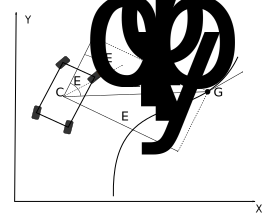
\includegraphics[height=4cm]{Figures/ptc_errors2.png} \label{fig:ptc_errors}}%
%	\hspace{0.1cm}
	\subfloat[]{\includegraphics[height=4cm]{Figures/fuzzy_ptc_inside.png}	\label{fig:ptc}}%
	\caption{(a) The deviation errors between robot pose and goal pose and (b) the fuzzy path tracking controller.}
	\label{fig:ptc_and_errors}
\end{figure}

\begin{figure}[!ht]
	\centering
	\subfloat[$E_o$, $E_\alpha$]{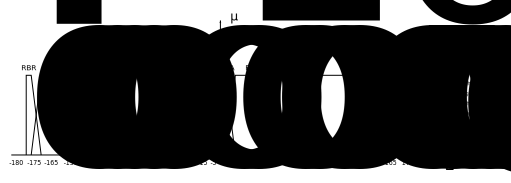
\includegraphics[width=\columnwidth]{Figures/eo_ea_mf.png}}\\%
	\subfloat[$E_p$]{\includegraphics[height=2.5cm]{Figures/ep_mf.png}}%
	\hspace{0.01cm}
	\subfloat[$E_y$]{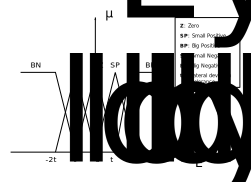
\includegraphics[height=2.5cm]{Figures/ey_mf.png}}%
	\hspace{0.01cm}
	\subfloat[$Direction$]{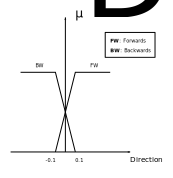
\includegraphics[height=2.5cm]{Figures/direction_mf.png}}\\%
	\caption{The membership functions of the input variables of the controller.}
	\label{fig:input_mfs}
\end{figure}	

\begin{figure}[!ht]
	\centering
	\subfloat[$speed$ $(v)$]{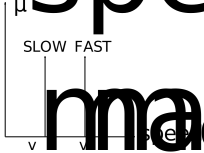
\includegraphics[height=2.5cm]{Figures/speed_mf.png}}%
	\hspace{0.2cm}
	\subfloat[$FSA$ $(\delta_f)$, $RSA$ $(\delta_r)$]{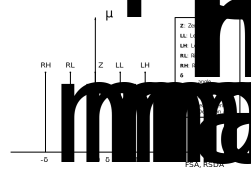
\includegraphics[height=2.5cm]{Figures/df_dr_mf.png}}%	
	\caption{The membership functions of the output variables of the controller.}
	\label{fig:output_mfs}
\end{figure}


As shown in Fig. \ref{fig:ptc_and_errors}, the controller considers four error variables and in particular the orientation error $E_o$, the angular deviation error $E_\alpha$, the position error $E_p$ and the lateral deviation error $E_y$, as well as the direction of motion defined as forwards for $|E_\alpha| \leq 120^\circ$ and backwards for $|E_\alpha| > 120^\circ$, whose membership functions are presented in Fig. \ref{fig:input_mfs}. The path tracking controller, similarly to the controller presented in \cite{reactive_fuzzy_ptc}, consists of three individual fuzzy logic controllers (FLCs), responsible for the control of the speed $v$, the front steering angle $\delta_f$ and the rear steering deviation angle $\alpha_r$, the membership functions of which are shown in Fig. \ref{fig:output_mfs}.

The rule set of the FLCs (Table \ref{tab:fuzzy_rules}) was designed such that the robot performs position correction when it is far from the goal and orientation correction when it is close to the goal so that it reaches the final goal pose similarly to the approach in \cite{flc_thesis}. In addition, using the rear steering deviation controller, the robot uses counter steering when the position and angular deviation errors are big and crab steering in order to correct slight lateral deviations without significant increase in the orientation error.

\begin{table}[!ht]
  \centering
  \caption{Fuzzy Path Tracking Controller Rule Set}
  \label{tab:fuzzy_rules}
  \resizebox{0.88\columnwidth}{!}{%
  \begin{tabular}{| c | l |}
    \hline
    \rotatebox[origin=c]{90}{\;\textbf{Speed}\;} &
    \begin{tabular}{l}
      if Ep is CLOSE then Speed is SLOW\\
      if Ep is FAR then Speed is FAST\\
    \end{tabular}\\ \hline
    \rotatebox[origin=c]{90}{\textbf{FSA}} &
    \begin{tabular}{l}\\[-0.2cm]
      if Ep is FAR and Ea is RBL then FSA is  Z\\
      if Ep is FAR and Ea is RL then FSA is LH\\
      if Ep is FAR and Ea is SL then FSA is LH\\
      if Ep is FAR and Ea is FL then FSA is LL\\
      if Ep is FAR and Ea is FA then FSA is  Z\\
      if Ep is FAR and Ea is FR then FSA is RL\\
      if Ep is FAR and Ea is SR then FSA is RH\\
      if Ep is FAR and Ea is RR then FSA is RH\\
      if Ep is FAR and Ea is RBR then FSA is  Z\\
      if Ep is CLOSE and Direction is FW and Eo is SL then FSA is LH\\
      if Ep is CLOSE and Direction is FW and Eo is FL then FSA is LL\\
      if Ep is CLOSE and Direction is FW and Eo is FA then FSA is Z\\
      if Ep is CLOSE and Direction is FW and Eo is FR then FSA is RL\\
      if Ep is CLOSE and Direction is FW and Eo is SR then FSA is RH\\
      if Ep is CLOSE and Direction is BW and Eo is SL then FSA is RH\\
      if Ep is CLOSE and Direction is BW and Eo is FL then FSA is RL\\
      if Ep is CLOSE and Direction is BW and Eo is FR then FSA is LL\\
      if Ep is CLOSE and Direction is BW and Eo is SR then FSA is LH\\[0.05cm]
    \end{tabular}\\ \hline
    \rotatebox[origin=c]{90}{\textbf{RSDA}} &
    \begin{tabular}{l}\\[-0.2cm]
      if Eo is not FA and Eo is not FR and Eo is not FL then RSDA is Z\\
      if Direction is FW and Eo is FA and Ey is BP then RSDA is  Z\\
      if Direction is FW and Eo is FL and Ey is BP then RSDA is  Z\\
      if Direction is FW and Eo is FR and Ey is BP then RSDA is  Z\\
      if Direction is FW and Eo is FA and Ey is SP then RSDA is LH\\
      if Direction is FW and Eo is FL and Ey is SP then RSDA is LH\\
      if Direction is FW and Eo is FR and Ey is SP then RSDA is LH\\
      if Direction is FW and Eo is FA and Ey is  Z then RSDA is  Z\\
      if Direction is FW and Eo is FL and Ey is  Z then RSDA is  Z\\
      if Direction is FW and Eo is FR and Ey is  Z then RSDA is  Z\\
      if Direction is FW and Eo is FA and Ey is SN then RSDA is RH\\
      if Direction is FW and Eo is FL and Ey is SN then RSDA is RH\\
      if Direction is FW and Eo is FR and Ey is SN then RSDA is RH\\
      if Direction is FW and Eo is FA and Ey is BN then RSDA is  Z\\
      if Direction is FW and Eo is FL and Ey is BN then RSDA is  Z\\
      if Direction is FW and Eo is FR and Ey is BN then RSDA is  Z\\
      if Direction is BW and Eo is FA and Ey is BP then RSDA is  Z\\
      if Direction is BW and Eo is FL and Ey is BP then RSDA is  Z\\
      if Direction is BW and Eo is FR and Ey is BP then RSDA is  Z\\
      if Direction is BW and Eo is FA and Ey is SP then RSDA is LH\\
      if Direction is BW and Eo is FL and Ey is SP then RSDA is LH\\
      if Direction is BW and Eo is FR and Ey is SP then RSDA is LH\\
      if Direction is BW and Eo is FA and Ey is  Z then RSDA is  Z\\
      if Direction is BW and Eo is FL and Ey is  Z then RSDA is  Z\\
      if Direction is BW and Eo is FR and Ey is  Z then RSDA is  Z\\
      if Direction is BW and Eo is FA and Ey is SN then RSDA is RH\\
      if Direction is BW and Eo is FL and Ey is SN then RSDA is RH\\
      if Direction is BW and Eo is FR and Ey is SN then RSDA is RH\\
      if Direction is BW and Eo is FA and Ey is BN then RSDA is  Z\\
      if Direction is BW and Eo is FL and Ey is BN then RSDA is  Z\\
      if Direction is BW and Eo is FR and Ey is BN then RSDA is  Z\\[0.05cm]
    \end{tabular}\\ \hline
  \end{tabular}
  }
\end{table}


\section{Experimental Results} \label{sec:results}
This section presents a series of experiments that demonstrate the behaviour of the autonomous navigation and exploration capabilities of the developed robotic platform.

The path tracking experiments presented in Fig. \ref{fig:ptc_exp1}-\ref{fig:ptc_exp2} were conducted in the Gazebo 3D simulator, with a view to demonstrate the operation of the fuzzy path tracking controller. For this experiment, a feasible static global path was constructed, which the robot managed to track successfully in both cases by using both counter and crab steering in order to offset angular and distance errors so as to follow the path as close as possible.

\begin{figure}[!ht]
  \centering
  \subfloat[The SLAM map, global path (green) and trajectory (red))]{\includegraphics[width=0.8\linewidth]{Figures/zic_zac_room.png}}\\%
  \subfloat[Front and rear steering angles $\delta_f (blue), \delta_r (red)$]{\includegraphics[width=\linewidth]{Figures/fsa_rsa_1.png}}%
  \caption{Path tracking experiment in Gazebo.}
  \label{fig:ptc_exp1}
\end{figure}

\begin{figure}[!ht]
  \centering
  \subfloat[The SLAM map, global path (green) and trajectory (red))]{\includegraphics[width=\linewidth]{Figures/slope_room_path_and_traj3.png}}\\%
  \subfloat[Front and rear steering angles $\delta_f (blue), \delta_r (red)$]{\includegraphics[width=\linewidth]{Figures/fsa_rsa_3.png}}%	
  \caption{Path tracking experiment under high slippage in a perpendicularly inclined corridor.}
  \label{fig:ptc_exp2}
\end{figure}

The experiments presented in Fig. \ref{fig:rsband_path}- \ref{fig:rsband_exp} were conducted in the STDR 2D simulator and demonstrate the planning stages of the proposed autonomous navigation system, as well as its successful application for three distinct goal poses.

\begin{figure}[!ht]
	\centering
	\subfloat[Global Plan]{\frame{\includegraphics[width=0.32\linewidth]{Figures/rsband_global_2.png}}}%
	\hspace{0.05cm}
	\subfloat[Elastic Band]{\frame{\includegraphics[width=0.32\linewidth]{Figures/rsband_eband_2.png}}}%
	\hspace{0.05cm}
	\subfloat[Reeds-Shepp Band]{\frame{\includegraphics[width=0.32\linewidth]{Figures/rsband_rsband_2.png}}}%
	\caption{Demonstration of the planning stages of the proposed 4-Tier autonomous navigation system.}
  \label{fig:rsband_path}
\end{figure}

\begin{figure}[!ht]
  \centering
  \subfloat[$p_1$]{\includegraphics[width=0.33\linewidth]{Figures/p1.png}}%
  %	\hspace{0.03\linewidth}
  \subfloat[$p_2$]{\includegraphics[width=0.33\linewidth]{Figures/p3.png}}%
  %	\hspace{0.03\linewidth}
  \subfloat[$p_3$]{\includegraphics[width=0.33\linewidth]{Figures/p4.png}}%
  \caption{Autonomous navigation experiments using the proposed 4-Tier autonomous navigation system for three distinct goal poses in the map sparse\_obstacles of the STDR simulator. The green line denotes the global path and the red line, the trajectory of the robot.}
  \label{fig:rsband_exp}
\end{figure}

Finally, an autonomous exploration experiment with the actual PANDORA Monstertruck robot was conducted in the Computer Systems and Architecture Lab (CSAL) of the School of Electrical and Computer Engineering, AUTH, as presented in Fig. \ref{fig:exploration_exp}.

\begin{figure}[!ht]
  \centering
  \frame{\includegraphics[width=\linewidth]{Figures/exploration_exp.png}}%
  \caption{Autonomous exploration experiment of PANDORA Monstertruck in CSAL. The map was constructed using the CRSM SLAM algorithm and the executed trajectory is denoted by the red continuous line.}
  \label{fig:exploration_exp}
\end{figure}


\section{Conclusions} \label{sec:conclusions}
%OLD: In this paper, the software and hardware architecture for a 4WS4WD mobile robot was presented capable of successfully exploring unknown environments by utilizing SLAM, exploration and navigation algorithms with focus on the prosposed 4-Tier Navigation architecture containing a Dijkstra/A* global path planning, Elastic Band dynamic path modification, with Reeds-Shepp interpolation (Reeds-Shepp Band) and complemented with a fuzzy path tracking controller.

In this paper, an autonomous 4WS4WD car-like robot was presented with regards to both its hardware and software architecture. As demonstrated in the experimental results, autonomous navigation is accomplished using the proposed 4-Tier autonomous navigation system that plans a holonomic global path, deforms it dynamically using the proposed Reeds-Shepp Band algorithm so that it can be collision free and kinematically feasible and finally tracks it robustly using the proposed fuzzy path tracking controller utilizing both counter and crab steering. It was also demonstrated that the robot can autonomously explore and map a previously unknown environment by employing the proposed software architecture.

Further work could be done to improve the robustness, stability and safety of the navigation system by using a more deterministic Reeds-Shepp planner and by adding collision detection capabilities in the path tracking controller. In addition, through the employment of additional sensors and perception algorithms, the capabilities of the robot could be significantly increased regarding localization, mapping, rough terrain traversal and point of interest search.

% use section* for acknowledgment
\section*{Acknowledgment}
The authors would like to thank PANDORA Robotics of the Aristotle University of Thessaloniki for the equipment, source code and know-how provided for the development of the PANDORA Monstertruck robotic platform.


\bibliographystyle{IEEEtran}
\bibliography{references}
\end{document}

% Note that the IEEE typically puts floats only at the top, even when this
% results in a large percentage of a column being occupied by floats.
%\begin{figure}[!t]
%	\centering
%	\includegraphics[width=2.5in]{}
%	\caption{}
%	\label{}
%\end{figure}

%\begin{figure*}[!t]
%\centering
%\subfloat[]{\includegraphics[width=2.5in]{}%
%\label{}}
%\hfil
%\subfloat[]{\includegraphics[width=2.5in]{}%
%\label{}}
%\caption{}
%\label{}
%\end{figure*}

% Note that the IEEE does not put floats in the very first column
% - or typically anywhere on the first page for that matter. Also,
% in-text middle ("here") positioning is typically not used, but it
% is allowed and encouraged for Computer Society conferences (but
% not Computer Society journals). Most IEEE journals/conferences use
% top floats exclusively. 
% Note that, LaTeX2e, unlike IEEE journals/conferences, places
% footnotes above bottom floats. This can be corrected via the
% \fnbelowfloat command of the stfloats package.

% An example of a floating table. Note that, for IEEE style tables, the
% \caption command should come BEFORE the table and, given that table
% captions serve much like titles, are usually capitalized except for words
% such as a, an, and, as, at, but, by, for, in, nor, of, on, or, the, to
% and up, which are usually not capitalized unless they are the first or
% last word of the caption. Table text will default to \footnotesize as
% the IEEE normally uses this smaller font for tables.
% The \label must come after \caption as always.
%
%\begin{table}[!t]
%% increase table row spacing, adjust to taste
%\renewcommand{\arraystretch}{1.3}
% if using array.sty, it might be a good idea to tweak the value of
% \extrarowheight as needed to properly center the text within the cells
%\caption{An Example of a Table}
%\label{table_example}
%\centering
%% Some packages, such as MDW tools, offer better commands for making tables
%% than the plain LaTeX2e tabular which is used here.
%\begin{tabular}{|c||c|}
%\hline
%One & Two\\
%\hline
%Three & Four\\
%\hline
%\end{tabular}
%\end{table}
